\documentclass{article}
\usepackage[utf8]{inputenc}
\usepackage[total={6in, 9in}]{geometry}
\usepackage{amsmath}
\usepackage{graphicx}
\usepackage{subcaption}
\numberwithin{equation}{section}
\usepackage{enumerate}
\usepackage{url}
\usepackage{tcolorbox}
\usepackage{enumitem}
\setlist{noitemsep}


\title{Channel Flow Turbulence Modeling with Tensor Basis Neural Network}
\author{Rui Fang}
\date{\today}

\begin{document}

\maketitle

\section{Introduction}
This project aims to utilize a machine learning method proposed by Ling et al., the tensor basis neural network (TBNN), to learn a model for the Reynolds stress anisotropy tensor of a turbulent channel flow from the DNS data. 


% Basic steps: 
% Obtain velocity and velocity gradient data from DNS 
% Compute mean velocity and mean velocity gradient 
% Compute true anisotropy tensors 
% Train TBNN 
% (Optional) Coarse grain 

\section{Tensor basis neural network}

The TBNN is a deep learning approach to turbulence modeling which uses a multiplicative layer with an invariant tensor basis to embed Galilean invariance into the predicted anisotropy tensor (see Figure \ref{fig:tbnn}).
\begin{figure}[h]
    \centering
    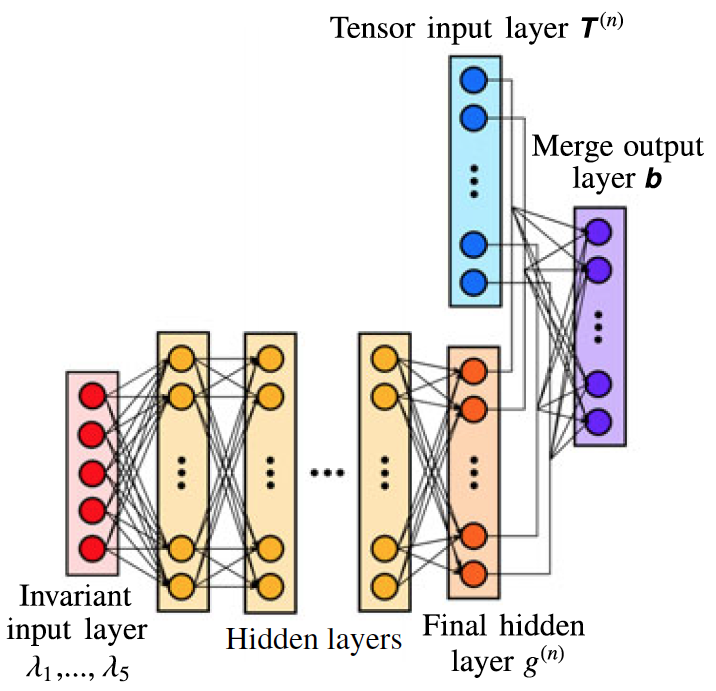
\includegraphics[width=0.4\linewidth]{TBNN.png}
    \caption{A diagram of the TBNN architecture \cite{ling2016reynolds}.}
    \label{fig:tbnn} 
\end{figure}

The relevant integrity basis was previously derived by Pope \cite{pope1975more}. Pope proved that in the most general incompressible case, the normalized Reynolds stress anisotropy tensor $\mathbf{b}$ that is a function of only $\mathbf{S}$ and $\mathbf{R}$ can be expressed as a linear combination of 10 isotropic basis tensors:
\begin{equation}
    \mathbf{b} = \sum_{n=1}^{10}g^{(n)}\left(\lambda_1, ..., \lambda_5\right) \mathbf{T}^{(n)},
    \label{eqn:tbnn}
\end{equation}
where $\mathbf{T}^{(1)}, ..., \mathbf{T}^{(10)}$ are the ten basis tensors, $g^{(1)}(\lambda_1, ... \lambda_5), ..., g^{(10)}(\lambda_1, ... \lambda_5)$ are the ten scalar coefficients, and $\lambda_1, ... \lambda_5$ are the five scalar invariants. The ten basis tensors and the five scalar invariants are known functions of $\mathbf{S}$ and $\mathbf{R}$ (see Eq.(\ref{eqn:basistensors}) and Eq.(\ref{eqn:invariants})), the non-dimensionalized mean strain rate and the mean rotation rate tensors, which are respectively the symmetric and asymmetric part of the mean velocity gradient $\nabla \langle \mathbf{U} \rangle$ multiplied by $k/\epsilon$. 

\begin{equation}
    \begin{split}
        \mathbf{T}^{(1)} &= \mathbf{S}\\
        \mathbf{T}^{(2)} &= \mathbf{SR}-\mathbf{RS}\\
        \mathbf{T}^{(3)} &= \mathbf{S}^2-\tfrac{1}{3}\mathbf{I}\cdot Tr(\mathbf{S}^2)\\
        \mathbf{T}^{(4)} &= \mathbf{R}^2-\tfrac{1}{3}\mathbf{I}\cdot Tr(\mathbf{R}^2)\\
        \mathbf{T}^{(5)} &= \mathbf{RS}^2-\mathbf{S}^2\mathbf{R}\\
    \end{split}
    \quad
    \begin{split}
        &\mathbf{T}^{(6)} = \mathbf{R}^2\mathbf{S}+\mathbf{S}\mathbf{R}^2-\tfrac{2}{3}\mathbf{I}\cdot Tr(\mathbf{SR}^2)\\
        &\mathbf{T}^{(7)} = \mathbf{R}\mathbf{S}\mathbf{R}^2-\mathbf{R}^2\mathbf{S}\mathbf{R}\\
        &\mathbf{T}^{(8)} = \mathbf{S}\mathbf{R}\mathbf{S}^2-\mathbf{S}^2\mathbf{R}\mathbf{S}\\
        &\mathbf{T}^{(9)} = \mathbf{R}^2\mathbf{S}^2+\mathbf{S}^2\mathbf{R}^2-\tfrac{2}{3}\mathbf{I}\cdot Tr(\mathbf{S}^2\mathbf{R}^2)\\
        &\mathbf{T}^{(10)} = \mathbf{R}\mathbf{S}^2\mathbf{R}^2-\mathbf{R}^2\mathbf{S}^2\mathbf{R}\\
    \end{split}
    \label{eqn:basistensors}
\end{equation}

\begin{equation}
    \lambda_1 = Tr(\mathbf{S}^2), \quad
    \lambda_2 = Tr(\mathbf{R}^2), \quad
    \lambda_3 = Tr(\mathbf{S}^3), \quad
    \lambda_4 = Tr(\mathbf{R}^2\mathbf{S}), \quad
    \lambda_5 = Tr(\mathbf{R}^2\mathbf{S}^2)
    \label{eqn:invariants}
\end{equation}


Mapping Eq.(\ref{eqn:tbnn}) into a neural network architecture, the TBNN has two input layers: the scalar invariant input layer and the tensor input layer. The input invariants $\lambda$'s are transformed through multiple densely connected hidden layers to yield the coefficients $g^{(n)}$. Then the merge layer performs a linear combination of the input tensors $\mathbf{T}^{(n)}$ with the coefficients $g^{(n)}$ and output the anisotropy stress tensor $\mathbf{b}$. This architecture ensures that Eq.(\ref{eqn:tbnn}) is satisfied, hence guaranteeing the Galilean invarianve of the predictions. 

In the following work, we make use of the TBNN package\footnote{\url{https://github.com/tbnn/tbnn}} in python to implement the TBNN approach. 

\section{Data sets}

We will train, validate and test the TBNN on a channel flow data set. The channel flow data is from a high-fidelity DNS in the Johns Hopkins Turbulence Database (JHTDB) \cite{li2008public}. In this project, the DNS data is used to provide the truth labels for the anisotropy tensors, and the coarse-grained DNS data are used as inputs to the neural network. This is to imitate the RANS data, which are not available in our situation. If the DNS data are directly used as inputs, then ideally the predicted and true anisotropy tensors should be identical given that the TBNN are successfully trained.

The JHTDB channel flow DNS is performed in a domain of size $8\pi \times 2 \times 3\pi $, using $2048\times512\times1536$ nodes, for approximately a single flow through time (corresponding to 4000 frames). In wall-parallel (x, z) directions, the grid spacing is uniform and the boundary conditions are periodic; in wall-normal (y) direction, the grid spacing is not uniform, and no-slip conditions are applied at the boundaries. Using a python interface\footnote{\url{https://github.com/idies/pyJHTDB}}, we can make queries to obtain velocity and velocity gradient data at the simulation nodes of a particular frame from the database. It is too costly to get the data for all the nodes and frames to perform averaging. Hence we choose to only get data at part of the nodes and frames. A qualitative convergence analysis is carried out to determine how much data may be considered enough. 

For example, we are currently picking every node in y direction, 1 node per 25 nodes in x direction, and 1 node per 51 nodes in z direction, resulting in a total number of $82\times512\times31$ nodes. And we query for 40 time frames from frame 0 to 3999 (frame indices: 99, 199, 299, ..., 3899, 3999). All these data are averaged over time and x-z plane to obtain the mean velocity $\langle\mathbf{U}\rangle$ and mean velocity gradient $\nabla\langle\mathbf{U}\rangle$. Based on these, we can calculate the Reynolds stresses $\langle u_i u_j\rangle$, the turbulent kinetic energy $k$, the normalized anisotropy stress tensors $b_{ij}$, the dissipation rate $\epsilon$, the wall shear stress $\tau_w$, the friction velocity $u_{\tau}$ and the viscous length scale $\delta_{\nu}$. Profiles of the mean velocity, Reynolds stresses and normalized anisotropy tensors in viscous units are shown in Figure \ref{fig:profiles_40}. In comparison, Figure \ref{fig:profiles_all} shows the profiles averaged over all time frames and all nodes in x-z plane. The true profiles are directly downloaded from the database website. By comparing the two figures, we observe that the profiles of our current data set are indeed converging to the true profiles. However, the Reynolds stresses profile and the normalized anisotropy tensors profile are not smooth enough. To improve it, we need to accumulate more data in future. 


\begin{figure}[h]
    \centering
    \begin{subfigure}{1.0\textwidth}
        \centering
        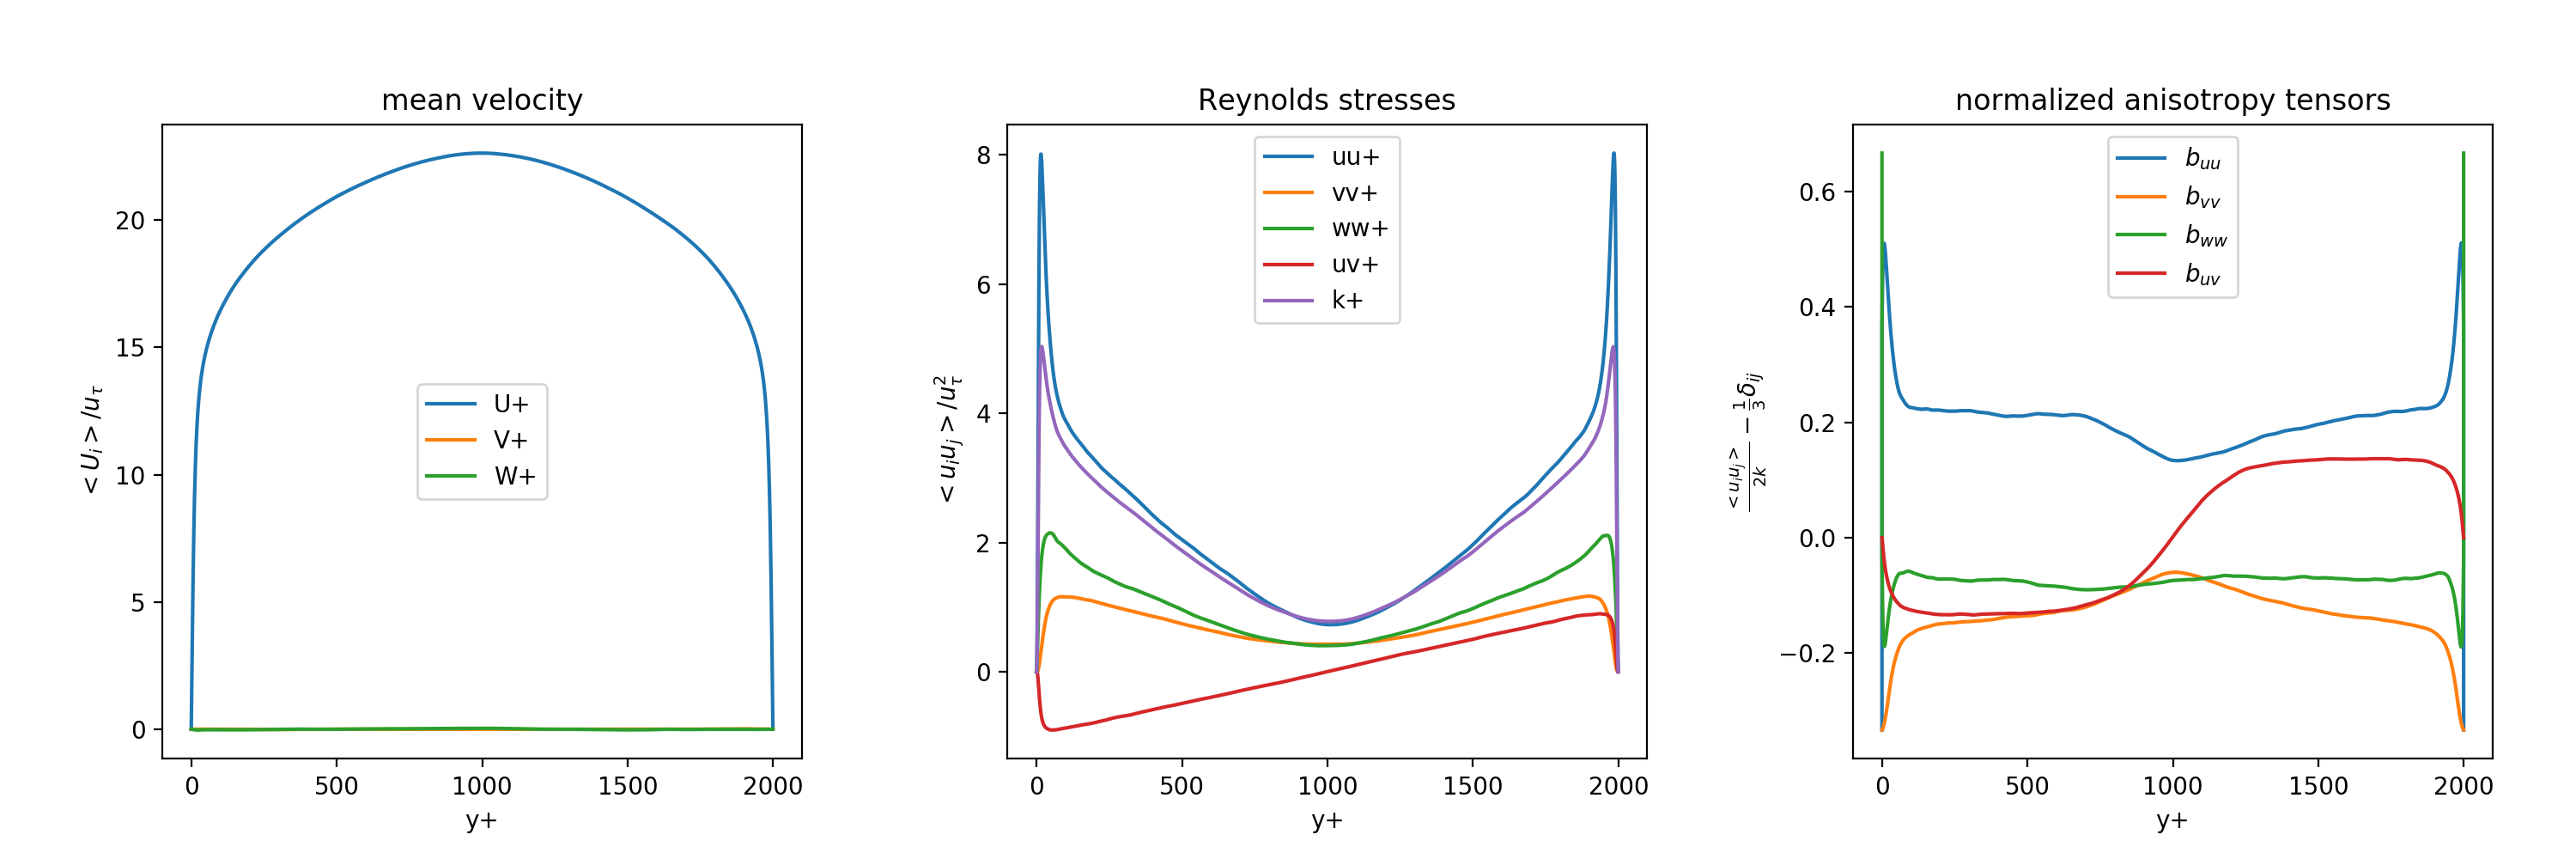
\includegraphics[width=0.95\linewidth]{profiles_40frames.png}
        \caption{averaged over 40 frames and $82\times512\times31$ nodes}
        \label{fig:profiles_40}
    \end{subfigure}
    \begin{subfigure}{1.0\textwidth}
        \centering
        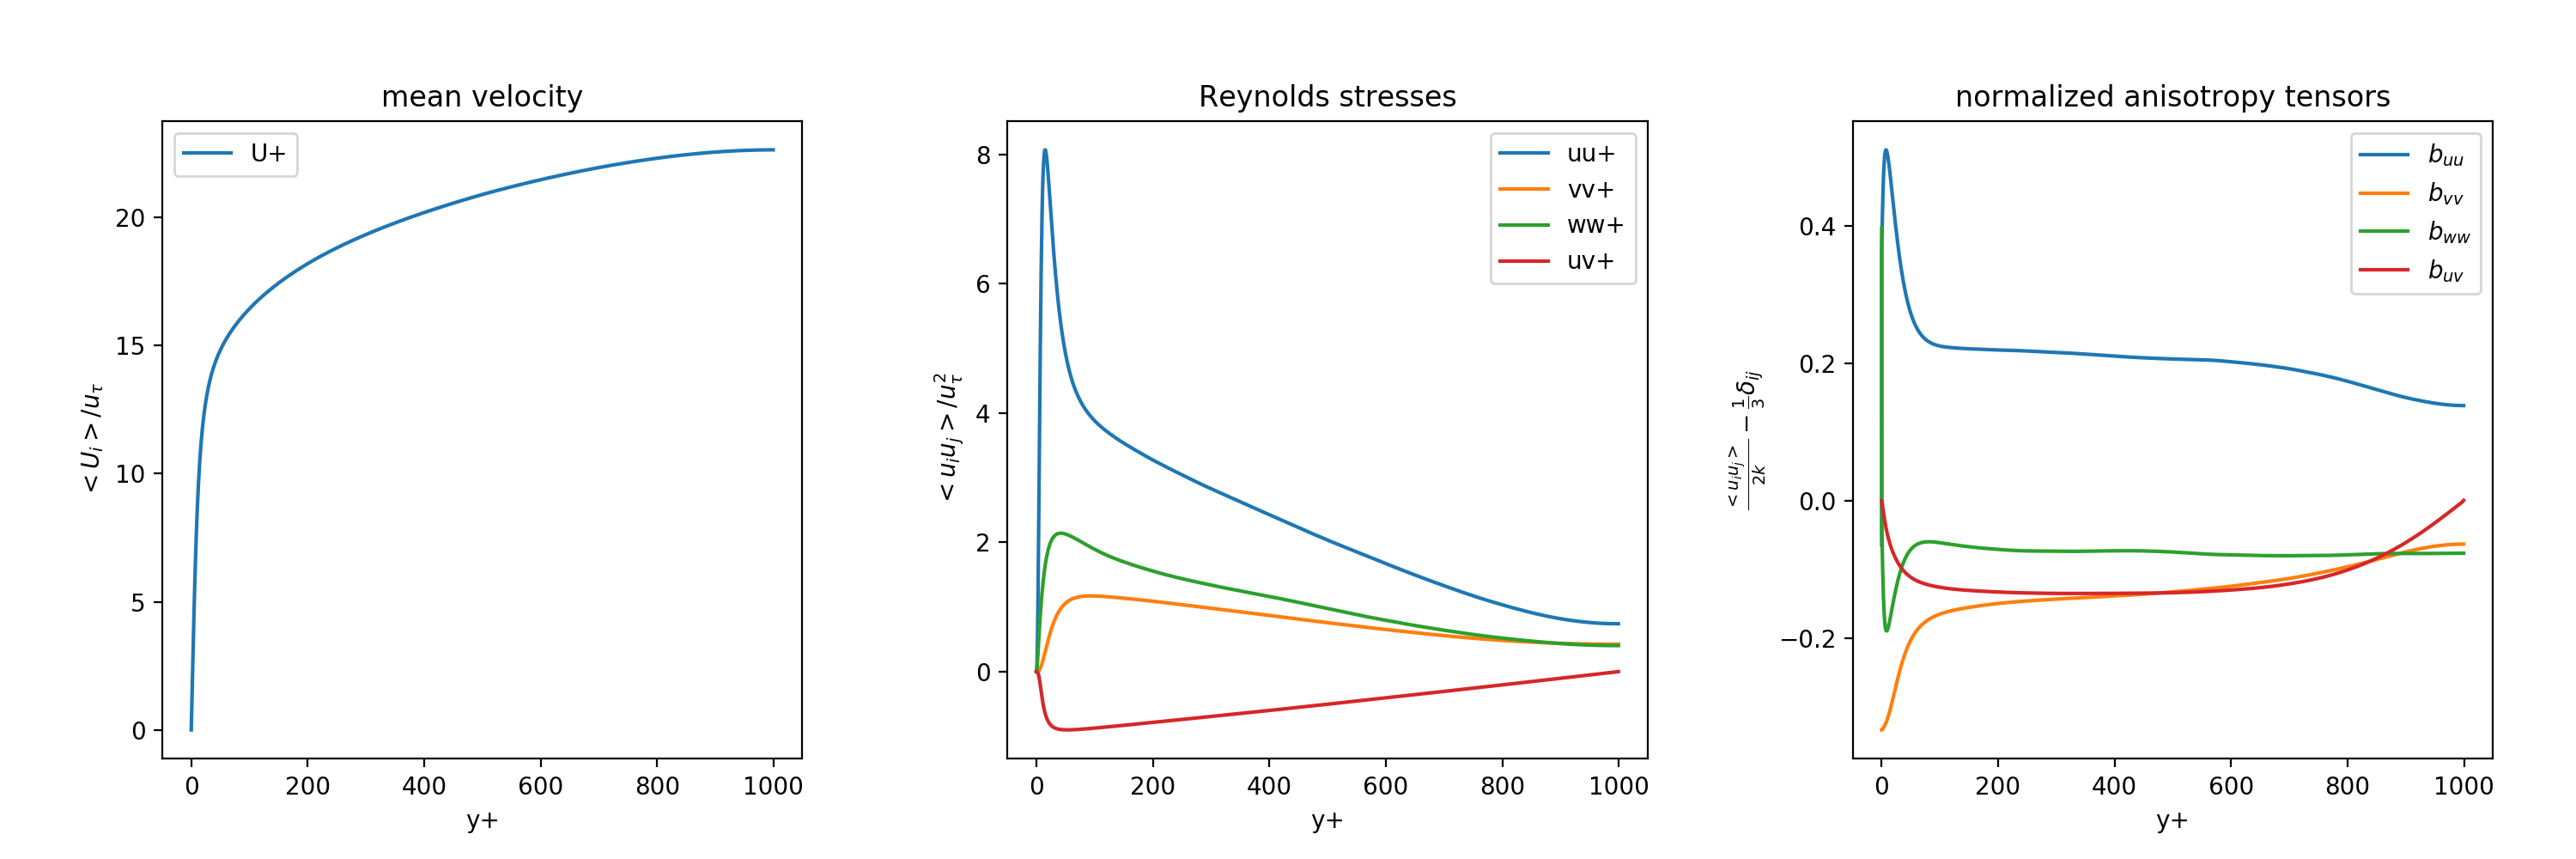
\includegraphics[width=0.95\linewidth]{profiles_entireDNS.png}
        \caption{averaged over 4000 frames and $2048\times512\times1536$ nodes}
        \label{fig:profiles_all}
    \end{subfigure}
    \caption{Channel flow profiles of mean velocity, Reynolds stresses and normalized anisotropy stress tensors in viscous units from two sets of data}
    \label{fig:profiles}
\end{figure}

The inputs to the neural network are the coarse-grained mean velocity gradient $\nabla\langle\mathbf{U}\rangle$, turbulent kinetic energy $k$ and the dissipation rate $\epsilon$. The coarse-graining procedure is basically reducing the data by averaging every $n$ points to represent a single point of the $n$ points. For example, there are originally 512 sample points along y direction. Choosing $n=3$, then 170 points will remain after coarse-graining. The y positions and truth labels of these points correspond to the original data of the 2nd, 5th, 8th, ... points of the 512 points. 

\section{Experiment}

The loss function associated with the TBNN is the mean squared error evaluated for all training samples and all 9 components of $\mathbf{b}$: 

\begin{equation}
    \text{Loss} = \frac{1}{9N}\sum_{m=1}^{N}\sum_i^3\sum_j^3\left(b_{ij,m,DNS}-b_{ij,m,TBNN}\right)^2.
    \label{eqn:loss}
\end{equation}

In this particular model, the hidden units of the hidden layers are chosen to be leaky ReLU. So at each node, the node input $\mathbf{x}$ is transformed to $f(\mathbf{x})=\text{max}(0, \mathbf{w}^T\mathbf{x}) + \alpha\cdot\text{min}(0,\mathbf{w}^T\mathbf{x})$, where the leakiness $\alpha$ is set to be $0.1$. The parameters to be trained in this model are the node weights $w$'s. The hyperparameters are the number of hidden layers, the number of nodes per hidden layer, the learning rate of the optimization algorithm, etc. 

The network is trained using the mini-batch stochastic gradient descent (SGD). The learning rate of this algorithm is controlled by three parameters: the initial learning rate, the decay rate, and the minimum learning rate. At the beginning of each epoch while doing the SGD, the learning rate is lowered by multiplying with the decay rate, until it hits the minimum learning rate. The batch size of this algorithm is also free to adjust.  

The TBNN implementation uses a basic early stopping technique to determine when to stop training. This is described as follows \cite{prechelt1998early}:  
\begin{enumerate}
    \item Split the training data into a training set and a validation set, e.g. in a 2-to-1 proportion.
    \item Train only on the training set and evaluate the per-example error on the validation set once in a while, e.g. after every fifth epoch.
    \item Stop training as soon as the error on the validation set is higher than it was the last time it was checked.
    \item Use the weights the network had in that previous step as the result of the training run.
\end{enumerate}

In actual implementation, extra parameters such as minimum and maximum number of epochs are also used. 

After the model is trained, we need to validate the model/optimize hyperparameters using the validation data set. Currently, this search is done by hand. The entire training and validation procedure is summarized below. 

\begin{tcolorbox}

\textbf{\textit{Before training}}
\begin{enumerate}
    \item For each sample: calculate $S_{ij}$, $R_{ij}$ from $\nabla\langle\mathbf{U}\rangle$, $k$, $\epsilon$; calculate scalar invariants, tensor basis from $S_{ij}$, $R_{ij}$; calculate true anisotropy tensor $b_{ij}$ from Reynolds stress tensor. 
    \item Split data into training, validation, test sets.
\end{enumerate}

\textbf{\textit{Training}}
\begin{enumerate}
    \item Define network structure: \texttt{num\_layers}, \texttt{num\_nodes}. 
    \item Specify loss function. Define \texttt{batch\_size}, \texttt{init\_learning\_rate}, \texttt{learning\_rate\_decay}, \texttt{min\_learning\_rate}, \texttt{max\_epochs}, \texttt{min\_epochs}, \texttt{interval}, and \texttt{average\_interval}.
    \item Perform SGD. In each epoch: 
    \begin{itemize}
        \item Set learning rate. 
        \item Do a full pass over the training data, update the weights of the neural networks.
        \item Check for early stopping criteria once per \texttt{interval} epochs.
        \begin{itemize}
            \item If epoch $\leq$ \texttt{min\_epochs}, continue.
            \item If epoch $>$ \texttt{max\_epochs}, stop.
            \item If \texttt{min\_epochs} $<$ epoch $\leq$ \texttt{max\_epochs}, check if the averaged validation error over \texttt{average\_interval} starts rising. If rises, then stop. 
        \end{itemize}
    \end{itemize}
\end{enumerate}

\textbf{\textit{Validation}}
\begin{enumerate}
    \item Tune hyperparameters and train the network until validation set yields best results.
\end{enumerate}

\end{tcolorbox}


\section{Results and Discussion}

We repeat the experiment for two groups of data: 1) 512 samples, without coarse-graining; 2) 170 samples, with coarse-graining. The lists of hyperparameters used are presented in Table \ref{tab:hyperparam_group1} and Table \ref{tab:hyperparam_group2} respectively for group 1 and group 2. 

For each group, we plot the training and validation error curves to visualize how the RMSE evolves over epochs for training and validation sets (Figure \ref{fig:convergence_group1}, \ref{fig:convergence_group2}). The RMSE is defined as the squared root of the loss: 
\begin{equation}
    \text{RMSE} = \sqrt{\frac{1}{9N}\sum_{m=1}^{N}\sum_i^3\sum_j^3\left(b_{ij,m,DNS}-b_{ij,m,TBNN}\right)^2}.
\end{equation}

Through a final RMSE report (Figure \ref{fig:output_group1}, \ref{fig:output_group2}), the performance of the TBNN model is compared with a baseline linear eddy viscosity model (LEVM). We can conclude from the test data RMSE that the TBNN predictions are more accurate than the LEVM predictions for both groups of data. In addition, the discrepancy between the accuracy of two models is larger in group 1 than that in group 2. 

We can discover more details by looking at individual components of $\mathbf{b}$. In Figure \ref{fig:b_vs_y_group1} and Figure \ref{fig:b_vs_y_group2}, the predictions and true values of four non-zero components of $\mathbf{b}$ are shown: $\mathbf{b}_{uu}$, $\mathbf{b}_{vv}$, $\mathbf{b}_{ww}$, $\mathbf{b}_{uv}$. Overall, the TBNN performs better than the LEVM. For $uu$, $vv$, and $ww$ components, the LEVM fails to capture the shape of the anisotropy completely, while the TBNN predicts the near wall portions pretty well but not so well in the center of the channel. For $uv$ component, the TBNN predictions look completely overlapping with the true values, showing very high accuracy, while the LEVM predicts the correct trend but the magnitudes are off as it gets closer to the walls. These observations hold for both groups. Comparing groups, the TBNN performs a lot better in group 1 than in group 2. 


\begin{table}[h]
    \parbox{.45\linewidth}{
        \centering
        \begin{tabular}{|l|r|}
        \hline
        number of hidden layers & 10 \\ \hline
        number of nodes per hidden layer & 15 \\ \hline
        batch size & 50 \\ \hline
        initial learning rate & 0.005 \\ \hline
        learning rate decay & 1 \\ \hline
        minimum learning rate & $10^{-6}$ \\ \hline
        minimum epoch & 100 \\ \hline
        maximum epoch & 2000 \\ \hline
        interval & 5 \\ \hline 
        average interval & 10 \\ \hline 
        \end{tabular}
        \caption{Group 1 hyperparameters}
        \label{tab:hyperparam_group1}
    }
    \hfill
    \parbox{.45\linewidth}{
        \centering
        \begin{tabular}{|l|r|}
        \hline
        number of hidden layers & 10 \\ \hline
        number of nodes per hidden layer & 15 \\ \hline
        batch size & 20 \\ \hline
        initial learning rate & 0.001 \\ \hline
        learning rate decay & 1 \\ \hline
        minimum learning rate & $10^{-6}$ \\ \hline
        minimum epoch & 50 \\ \hline
        maximum epoch & 2000 \\ \hline
        interval & 2 \\ \hline 
        average interval & 4 \\ \hline 
        \end{tabular}
        \caption{Group 2 hyperparameters}
        \label{tab:hyperparam_group2}
    }
\end{table}


\begin{figure}[h]
    \centering
    \begin{subfigure}{0.6\textwidth}
        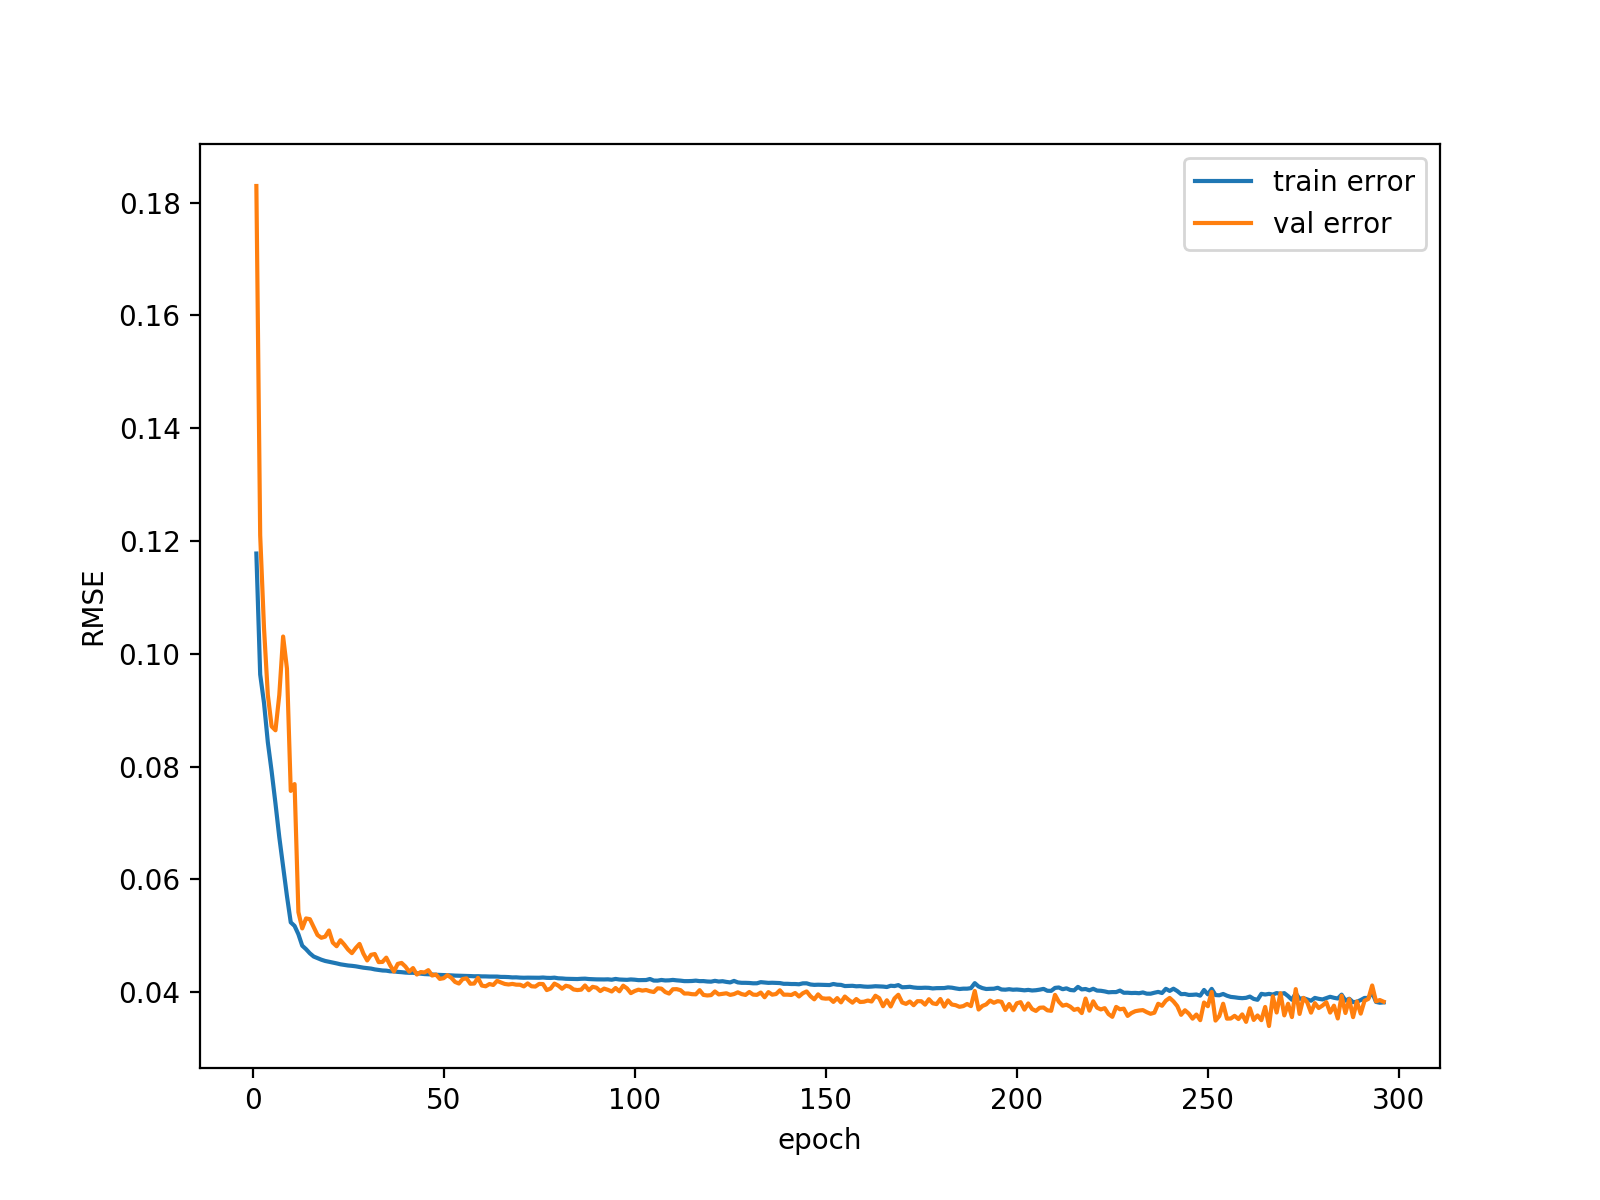
\includegraphics[width=1.0\linewidth]{results/512samples/convergence.png}
        \caption{Training and validation error curves}
        \label{fig:convergence_group1}
    \end{subfigure}
    \begin{subfigure}{0.33\textwidth}
        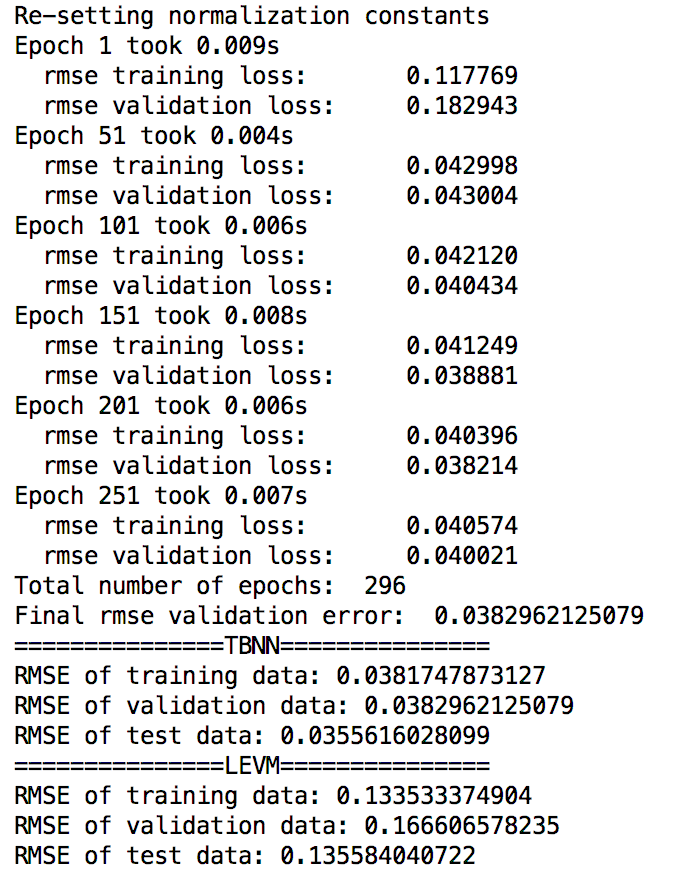
\includegraphics[width=1.0\linewidth]{results/512samples/output.png}
        \caption{Final RMSE report}
        \label{fig:output_group1}
    \end{subfigure}
    \caption{Group 1 results}
    \label{fig:results_group1}
\end{figure}

\begin{figure}[h]
    \centering
    \begin{subfigure}{0.6\textwidth}
        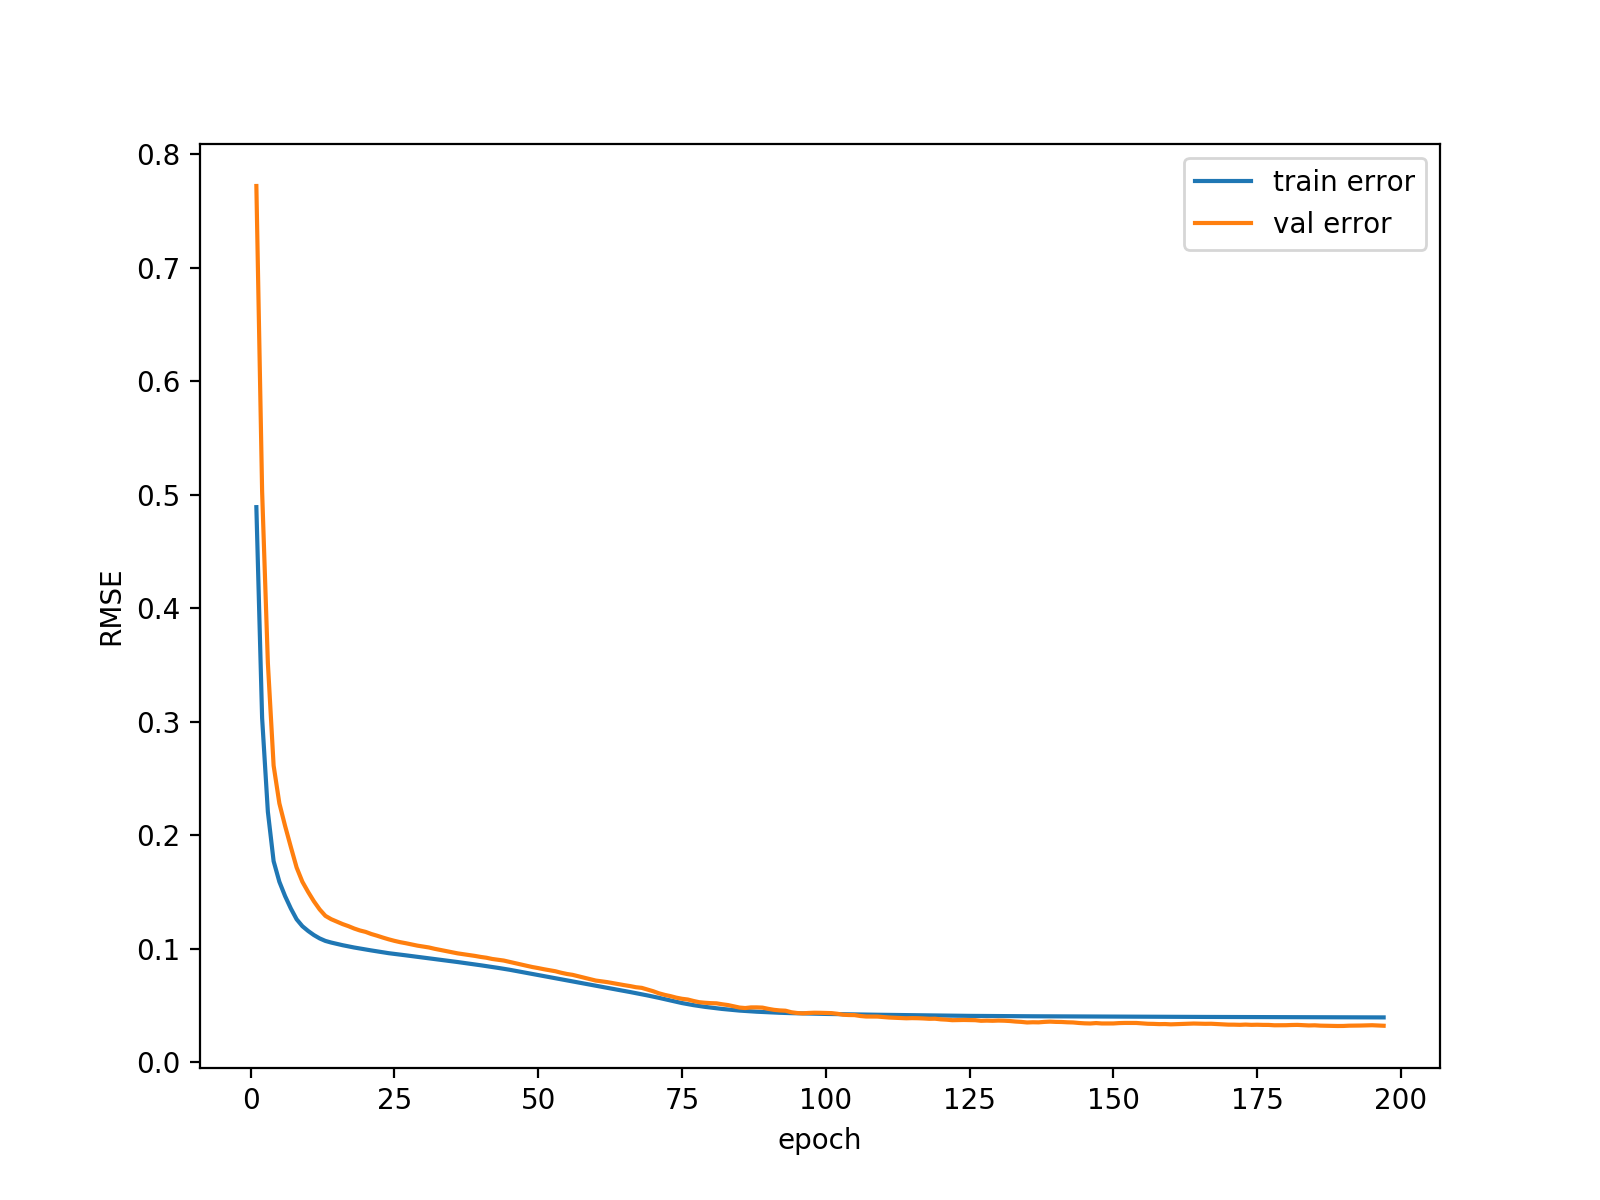
\includegraphics[width=1.0\linewidth]{results/170samples/convergence.png}
        \caption{Training and validation error curves}
        \label{fig:convergence_group2}
    \end{subfigure}
    \begin{subfigure}{0.38\textwidth}
        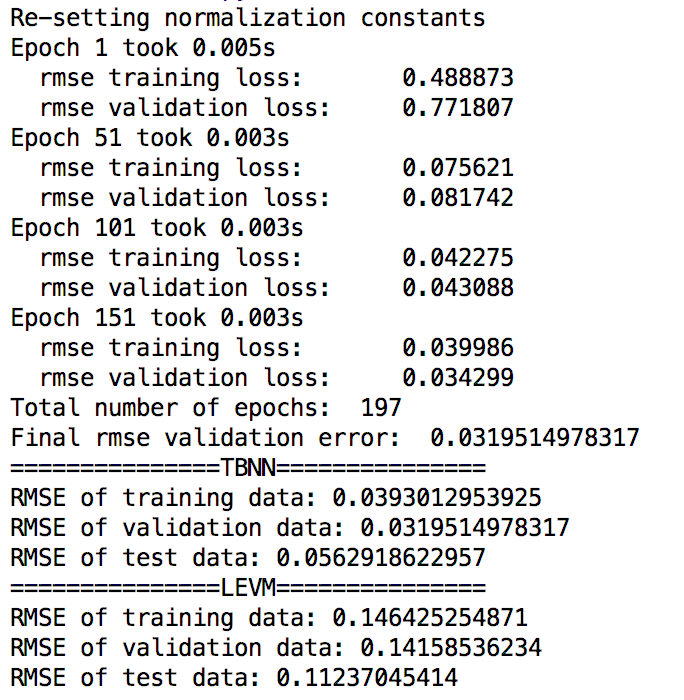
\includegraphics[width=1.0\linewidth]{results/170samples/output.png}
        \caption{Final RMSE report}
        \label{fig:output_group2}
    \end{subfigure}
    \caption{Group 2 results}
    \label{fig:results_group2}
\end{figure}

\begin{figure}[h]
    \centering
    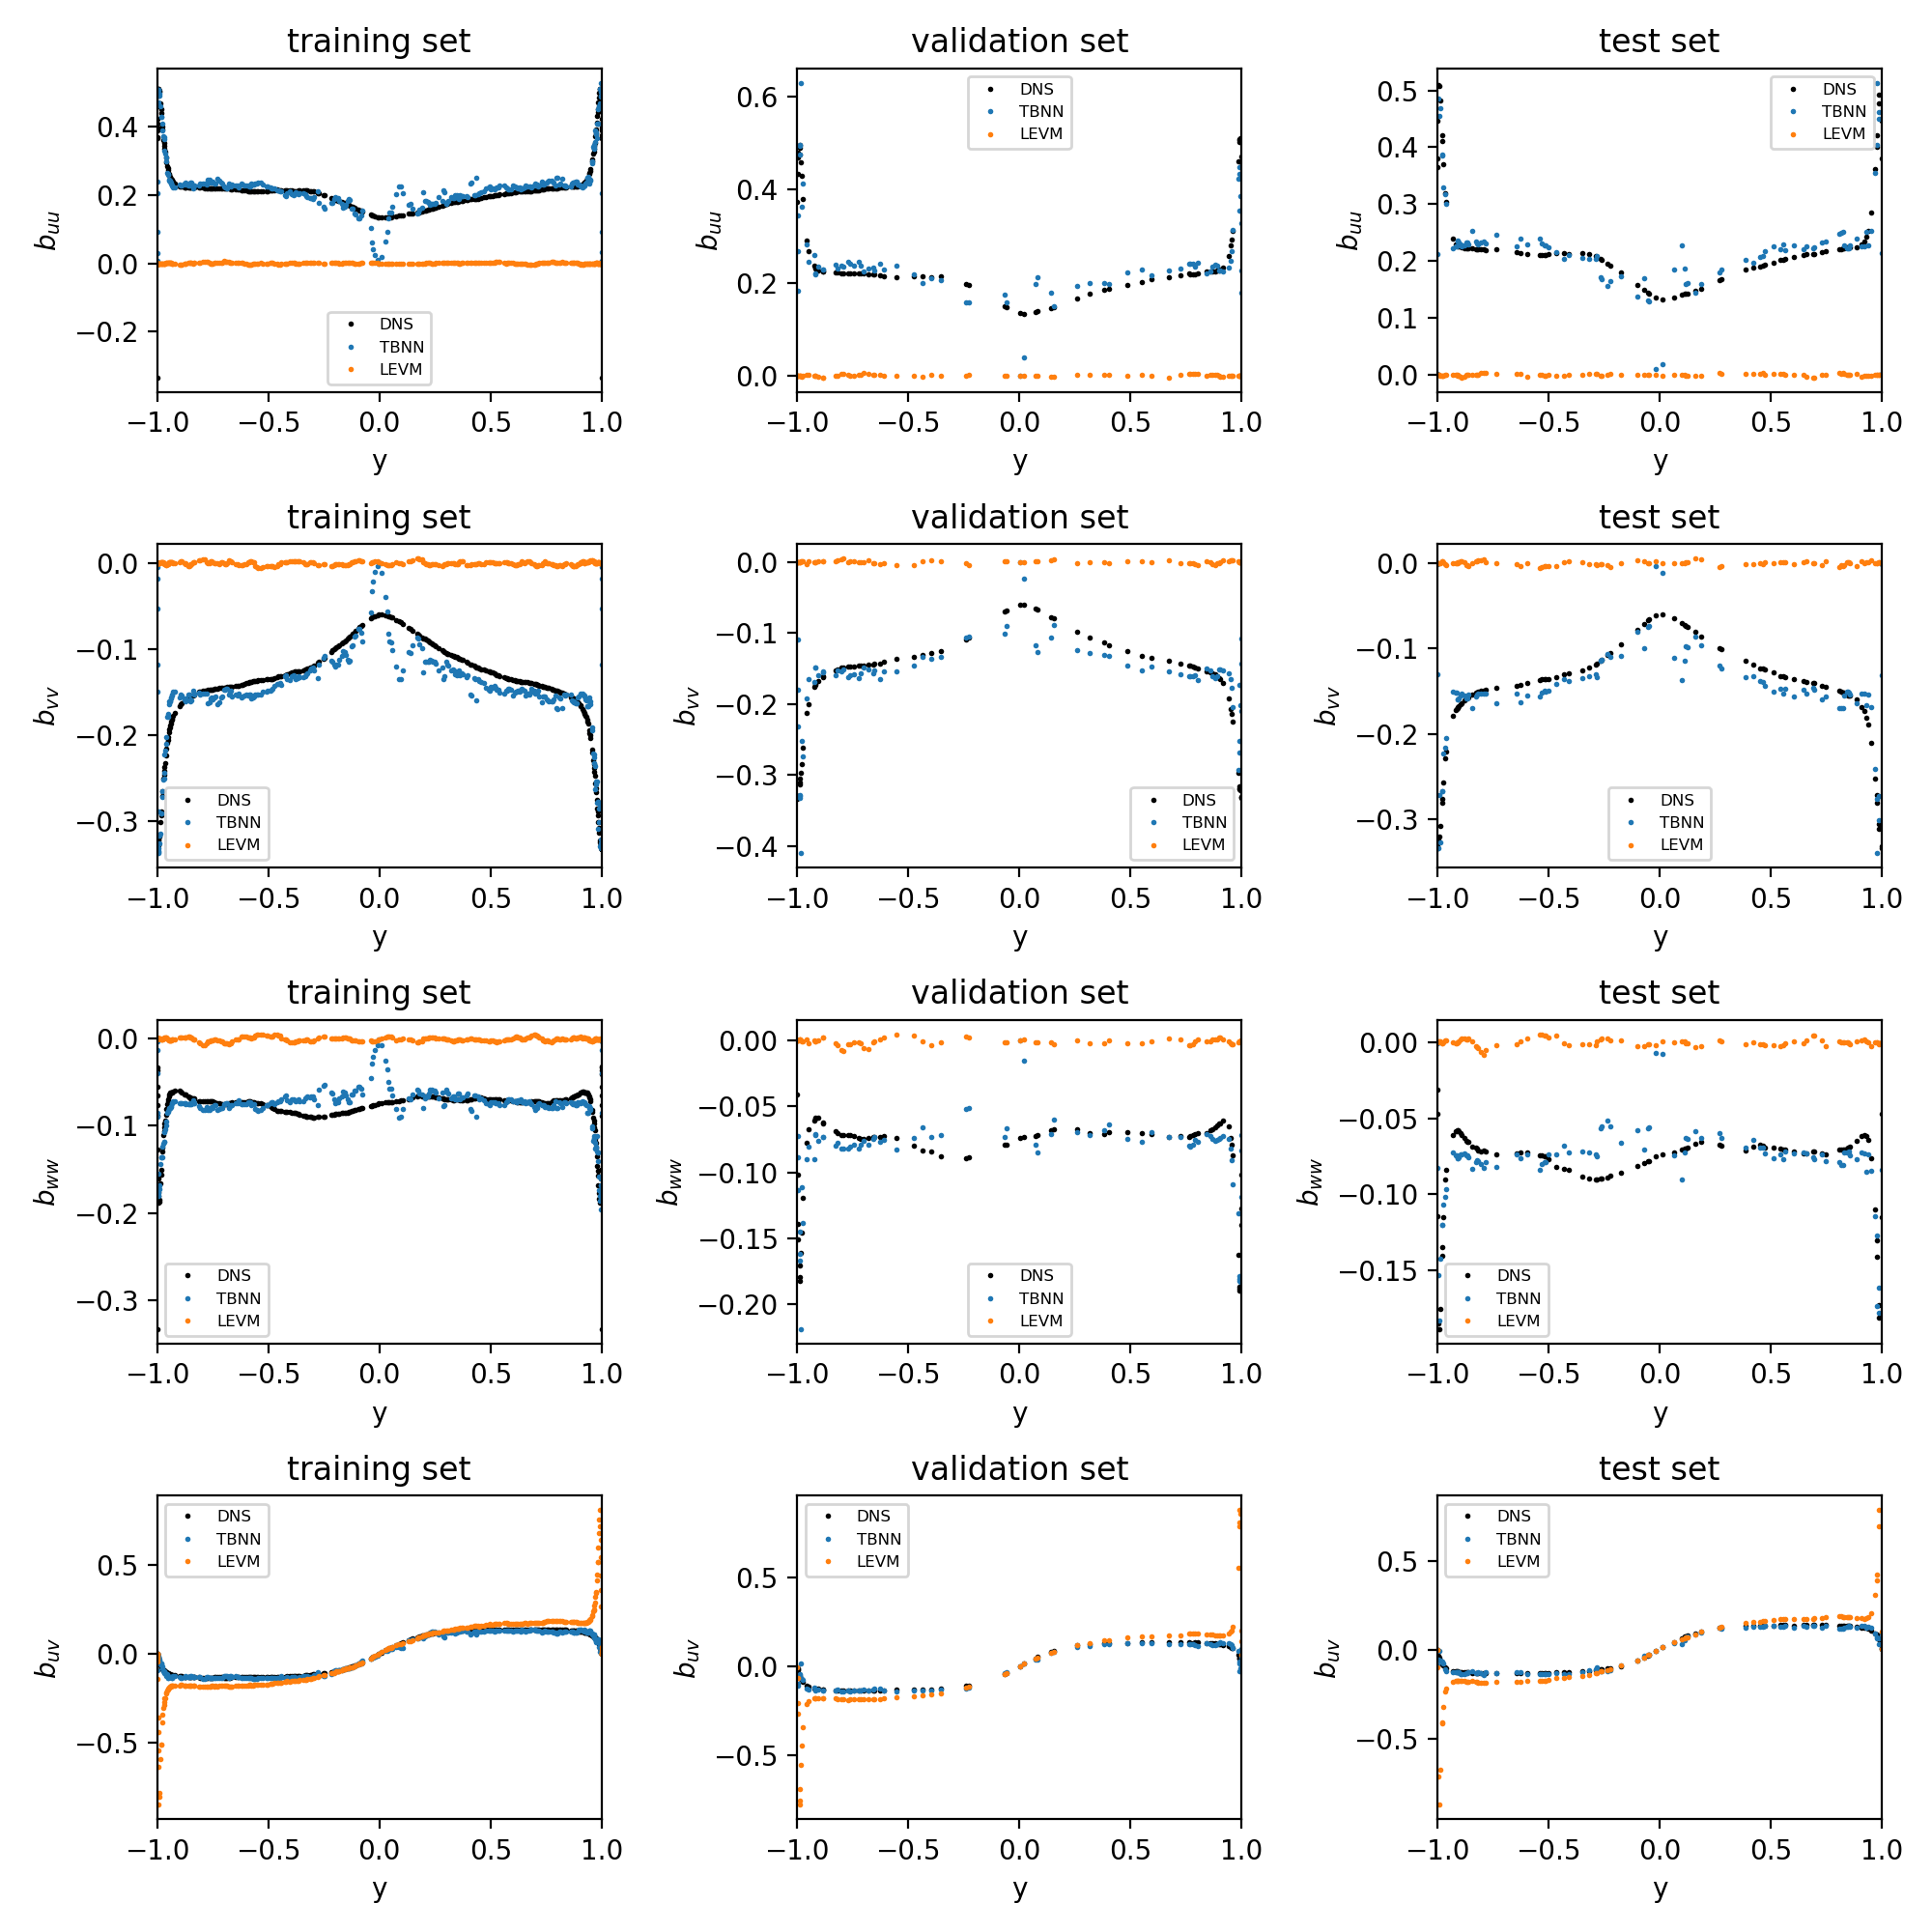
\includegraphics[width=1.0\linewidth]{results/512samples/b_vs_y.png}
    \caption{Group 1: True values, TBNN and LEVM predictions of anisotropy tensors vs y position (uu, vv, ww, and uv components of $\mathbf{b}$)}
    \label{fig:b_vs_y_group1}
\end{figure}

\begin{figure}[h]
    \centering
    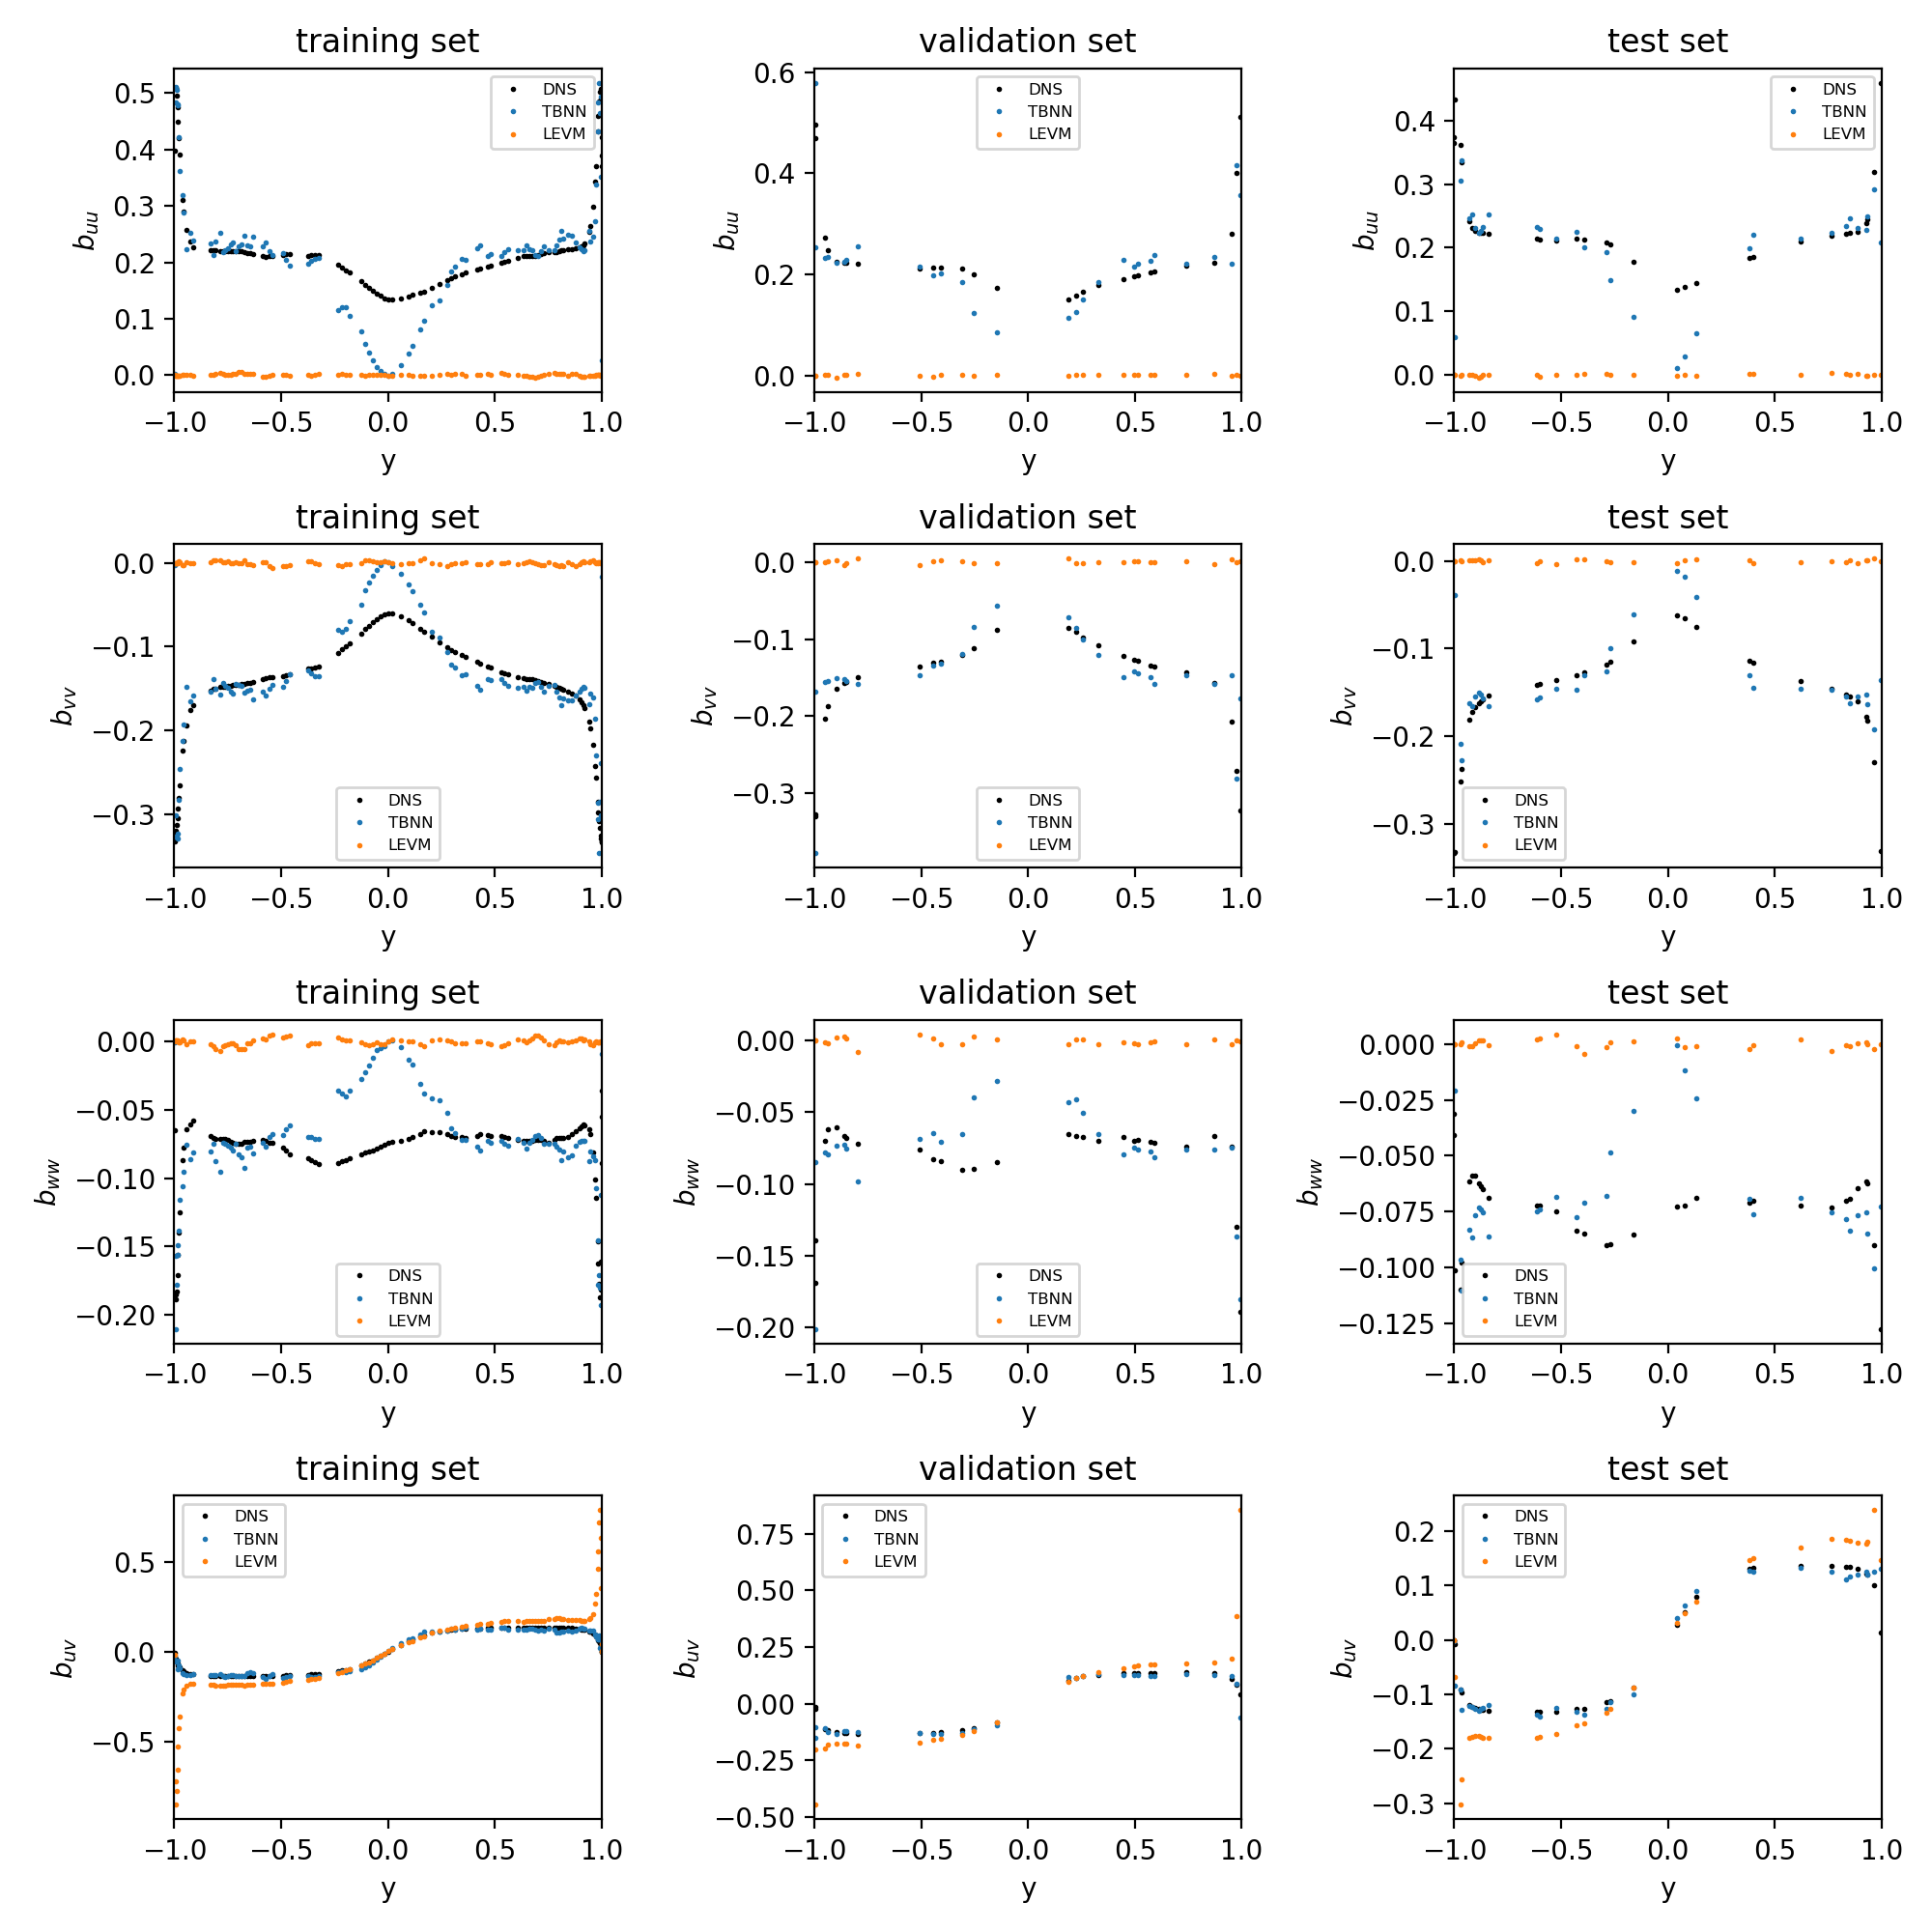
\includegraphics[width=1.0\linewidth]{results/170samples/b_vs_y.png}
    \caption{Group 2: True values, TBNN and LEVM predictions of anisotropy tensors vs y position (uu, vv, ww, and uv components of $\mathbf{b}$)}
    \label{fig:b_vs_y_group2}
\end{figure}

\section{Conclusion}

Based on the results, the capability of the TBNN to make relatively good predictions of the anisotropy tensors is confirmed. However, the fact that the TBNN tends to predict wrong values in the center of channel for $uu$, $vv$, and $ww$ components raises up new questions. 

The next steps focus on improving the neural network performance from two aspects. First, since we partition the data set into three sets, the training set may not be big enough for the neural network to learn the true model and the results may largely depend on a particular random choice of the training and validation sets. To resolve this, techniques such as cross validation will be helpful. Second, we hope to improve the process of optimizing hyperparameters. It is important to automate the search especially when the hyperparameter space is huge. We will try to implement Bayesian optimization to accomplish this. 


\bibliography{ref}
\bibliographystyle{plain}


    
\end{document}
